\documentclass[a4paper, 14pt]{extarticle}
\usepackage[english, russian]{babel}
\usepackage[utf8x]{inputenc}
\usepackage{fullpage}
\usepackage{indentfirst} % Первый абзац в разделе тоже с красной строки
\usepackage{cmap} % для кодировки шрифтов в pdf (чтобы не было крокозябры при копировании из pdf )
\usepackage{graphicx} % для вставки картинок
\graphicspath{{res/}} % Путь к папке с картинками
%\sloppy % Включение переноса слов в тексте
%\hyphenpenalty=10000 

\title{Фреймворк для конечно-разностного моделирования диффузионных задач на гибридных вычислительных кластерах}
\author{Фролов Даниил Александрович}

% Для красивой вставки исходного программного кода 
\usepackage{listings}
\usepackage{color}

\definecolor{mygreen}{rgb}{0,0.6,0}
\definecolor{mygray}{rgb}{0.5,0.5,0.5}
\definecolor{mymauve}{rgb}{0.58,0,0.82}

% Параметры раскрски исходного кода программы 
\lstset{ %
	language = Java,
	extendedchars=\true, %Чтобы русские буквы в комментариях были
	%inputencoding=cp1251,
	%commentstyle=\itshape,
	%stringstyle=\bf,
  backgroundcolor=\color{white},   % choose the background color
  basicstyle=\footnotesize,        % size of fonts used for the code
  %basicstyle=\ttfamily\fontsize{11pt}{11pt}\selectfont,
  breaklines=true,                 % automatic line breaking only at whitespace
  captionpos=b,                    % sets the caption-position to bottom
  commentstyle=\color{mygreen},    % comment style
  escapeinside={\%*}{*)},          % if you want to add LaTeX within your code
  keywordstyle=\color{blue},       % keyword style
  stringstyle=\color{mymauve},     % string literal style
}

\usepackage{hyperref} % Для добавления ссылок в тесте

% Настройка цветов для ссылок
\hypersetup{
colorlinks = true,
linkcolor = black,
pagecolor = black,
urlcolor = blue, 
citecolor = black
}

% Математика
\usepackage{amssymb} % For use "mathbb" function
\usepackage{amsmath}
\usepackage{amsthm}
\usepackage{mathrsfs}
\newcommand{\La}{\mathscr{L}} % Функция Лагранжа
\newcommand{\ls}{{ℓ}} % Красивая l, чтобы легче было отличить от i, 1 b других палок
\providecommand{\norm}[1]{\lVert#1\rVert} % Норма вектора : ||w||
\newcommand{\dpt}[1]{\left\langle#1\right\rangle} % dot product using brackets
\newcommand{\brackets}[1]{\left(#1\right)} % Обернуть скобками автоматического размера
%\newcommand{\dpts}[2]{#2 \langle#1 #2 \rangle} % dot product using brackets with manual size
\newcommand{\R}{\mathbb{R}} % beautiful R for R^n labels
\newcommand{\il}{i = 1, \ldots, \ls} % writes i = 1, ..., l
\newcommand{\ili}{\quad i = 1, \ldots, \ls} % writes i = 1, ..., l with indent in begin
\newcommand{\sumil}{\sum_{i=1}^{\ls}} % Сумма по i, которая изменяется от 1 до l
\newcommand{\minl}{\min\limits} % min with limits under "min" label
\newcommand{\maxl}{\max\limits} % max with limits under "max" label

% Окружение для теорем, определений и т.д.
\theoremstyle{definition}
\newtheorem{definition}{Определение}
\newtheorem{theorem}{Теорема}
\newtheorem{example}{Пример}

% Поправить стиль отрисовки формул (особенно актуально для сумм https://ru.sharelatex.com/learn/Display_style_in_math_mode)
\everymath{\displaystyle}

%\bibliographystyle{unsrt} % упорядочить список использованной литературы по порядку упоминания их в тексте
\bibliographystyle{utf8gost705u}
%\bibliographystyle{utf8gost71u}

\usepackage[labelfont=bf, labelsep=space]{caption} % Делаем надписи "Рис.1" под рисунками жирными и без двоеточия.
\usepackage[top=20mm, bottom=20mm, left=30mm, right=20mm
, nohead % Убрать расстояние для верхних колонтикулов
]
{geometry} % Размер полей у старницы
\setlength{\parindent}{1.25cm} % Размер интервала для абзацев 
\usepackage{setspace}
\singlespacing % одинарный интервал
\renewcommand\normalsize{\fontsize{14}{16.8pt}\selectfont} % Сделать размер шрифта 14

\usepackage{caption} % подписи к рисункам в русской типографской традиции
\DeclareCaptionFormat{GOSTtable}{#2#1\\#3}
\DeclareCaptionLabelSeparator{fill}{\hfill}
\DeclareCaptionLabelFormat{fullparents}{\bothIfFirst{#1}{~}#2}
\captionsetup[table]{
     format=GOSTtable,
     %font={footnotesize},
     labelformat=fullparents,
     labelsep=fill,
     labelfont=normal,
     textfont=bf,
     justification=centering,
     singlelinecheck=false
     }
     
% Начинать каждую главу с новой страницы
\usepackage{titlesec}
\newcommand{\sectionbreak}{\clearpage}

\begin{document}
\setcounter{tocdepth}{3}

{
\thispagestyle{empty}

\begin{center}
	
	Министерство образования и науки Российской Федерации\\[0.3cm]
	Государственное образовательное учреждение\\
	высшего профессионального образования\\
	"<Ярославский государственный университет им. П.Г. Демидова">\\
	(ЯрГУ)\\[0.3cm]
	
	Кафедра компьютерных сетей
	
	\bigskip
	
	\hspace{15em}"<Допустить к защите">
	
	\begin{flushright}
		Заведующий кафедрой\par
		д. ф.-м. н., профессор\par
		\underline{\hspace{3.2cm}}Глызин\,С.\,Д.\par
		"<\underline{\hspace{0.5cm}}">\underline{\hspace{3.4cm}}20\underline{\hspace{0.5cm}} г.\par
	\end{flushright}
	
	\bigskip
	
	{\textbf
		{\textit
			{Выпускная квалификационная работа бакалавра}
		}
	}
	\\
	по направлению 010500.62 Прикладная математика и информатика
	
	\bigskip
	
	{\bf
		Фреймворк для конечно-разностного моделирования диффузионных задач на гибридных вычислительных кластерах 
	}
\end{center}

\medskip

\begin{flushright}
	Научный руководитель\par
	д. ф.-м. н., профессор\par
	\underline{\hspace{3.5cm}}Глызин\,С.\,Д.\par
	"<\underline{\hspace{0.8cm}}">\underline{\hspace{3.5cm}}2015 г.\par
\end{flushright}

\bigskip 

\begin{flushright}
	Студент группы ИВТ-43-БО\par
	\underline{\hspace{2.5cm}}Фролов\,Д.\,А.\par
	"<\underline{\hspace{0.8cm}}">\underline{\hspace{3.5cm}}2015 г.\par
\end{flushright}

\vspace{\fill}

\begin{center}
	Ярославль 2015
\end{center}

\clearpage

}

\tableofcontents

\section*{Введение}

\par К классу диффузионных относятся такие задачи как уравнение теплопроводности или реакция Белоусова-Жаботинского.

\par Развитие современного общества зачастую ставит перед наукой цели, решение которых требует решения самых разнообразных систем дифференциальных уравнений. В том числе и систем диффузионных уравнений. К таким задачам можно отнести уравнение теплопроводности !!! (примеры других задач). Каждую из них можно решать с помощью численных методов, например, методом Эйлера, многошаговыми методами Рунге-Кутты или методами Дормана-Принса. Подобные вычисления удобно автоматизировать, чтобы в дальнейшем иметь возможность быстро производить расчеты.

\section{Постановка задачи}

\subsection{Теоретические основы решения диффузионных задач}

\par Как известно, в общем случае задачи реакции диффузии представимы в виде системы дифференциальных уравнений:
$$\frac{\partial u}{\partial t} = D \bigtriangleup u + F(u);$$
$$\frac{\partial u}{\partial v} = 0, F(0) = 0.$$

\par Для их решения применяются различные численные методы, в том числе метод Эйлера, метод Ругне-Кутты, Дормана-Принса. Все эти методы в той или иной степени могут быть использованы для численного решения задачи реакции диффузии. Кратко рассмотрим каждый из вышеперечисленных методов.

\par Метод Эйлера считается наиболее простым численным методом решения дифференциальных уравнений. Он относится к явным, одношаговым методам первого порядка точности и фактически основан на аппроксимации интегральной кривой кусочно-линейной функцией. Упрощенно метод Эйлера может быть представлен в виде формулы:
$$y_i = y_{i-1} + \bigtriangleup t \cdot f(t, y_{i-1}).$$

\par Второй метод, который может быть использован для решения поставленной задачи, -- метод Рунге-Кутты. Данный метод кратко описывается следующей схемой.

\par Пусть дана начальная задача Коши
$$\dot y = f(x, y)$$
и некоторое начальное условие
$$y(x_0) = y_0.$$

\par Тогда каждую последующую точку решения можно вычислить с помощью предыдущей, используя следующее равенство:
$$y_{n+1} = y_n + \sum_{i=0}^s b_i k_i.$$

\par Коэффициенты $k_i$ вычиляются, исходя из следующих соотношений:
$$k_1 = hf(x_n, y_n),$$
$$k_2 = hf(x_n + c_2 h, y_n + a_{21}k_1),$$
$$\cdots$$
$$k_s = hf(x_n + c_s, y_n + a_{s1}k_1 + a_{s2}k_2 + \cdots + a_{s,s-1}k_{s-1}).$$

\par Количество коэффицентов $k_i$ определяет порядок метода: к примеру, для четырехстадийной схемы Рунге-Кутты необходимо вычислить четрые таких коэффициента.

\par Для параметров $a_{ij}$, $b_i$, $c_i$, которые используются при расчеты $k_i$, должны выполняться следующие равенства:
$$\sum_{j=1}^{i-1}{a_{ij}} = c_i,$$
$$\sum_{j=1}^s{b_i} = 1,$$
$$0 \le (b_i, c_i, a_{ij}) \le 1,$$
$$b_i > 1.$$

\par Именно параметры $a_{ij}$, $b_i$ и $c_i$ задают конкретный метод Рунге-Кутты.

\par Как правило, для решения дифференциальных уравнений используются схемы невысоких порядков точности, поэтому в нашем случае достаточно воспользоваться четырехстадийной реализацией метода Рунге-Кутты, то есть взять $s = 4$.

\par Для решения задачи диффузии, как уже было сказано выше, также может быть использован метод Дормана-Принса, который фактически является модификацией метода Рунге-Кутты. По сравнению с последним он является более точным за счет большего числа стадий вычисления нового состояния. Среди особенностей метода также стоит отметить изменяемость шага вычислений.

\par Очевидно, что применение того или иного метода, оказывает влияние на точность и скорость производимых вычислений и, естественно, на конечный результат. В связи с этим, выбор конкретного метода решения следует оставить за пользователем.

\subsection{Основные требования к приложению}

\par Каждая конкретная задача диффузии, которая может быть поставлена конечным пользователем, характеризуется несколькими параметрами. Во-первых, это уравнение (или система уравнений), описыющее происходящий физический, химический или биологический процесс. Во-вторых, для решения задачи необходимо знать область, в которой этот процесс протекает. Назовем ее областью задачи. При этом необходимо учитывать, что область задачи может быть одномерной, двумерной или трехмерной и состоять из так называемых блоков. Для одномерного случая этими блоками являются отрезки, в случае плоскости - прямоугольники, а если область трехмерна - параллелепипеды. Каждый из блоков характеризуется координатами в пространстве и размерами, а также информацией о своих границах. Информация о границе блока содержит данные о поведении функции, которая моделирует процесс, в граничных точках. В качестве краевых условий могут использоваться условия Неймана или условия Дирихле. В первом случае задается поведение производной функции в граничных точках, а во втором - конкретные значения функции, заданные, возможно, с помощью другой функции. Следует заметить, что на разные участки границы могут быть наложены разные краевые условия. Область задачи может состоять из нескольких частей. Эти части, или блоки, могут иметь общую границу, точнее, место соединения. В этом случае на данный участок блоков не распространяются условия, заданные на границе, а место соединения считается внутренней областью.

\par На рисунке !!! представлен пример двумерной области, в которой моделируется уравнение теплопроводности. Указанная область состоит из двух прямоугольников, соединенных между собой. Место соединения обозначено пунктирной линией. Красным цветом выделена часть границы, на которой заданы условия Неймана с отрицательной производной, синим - условия Дирихле, зеленым - условия Неймана с положительной производной. На всей остальной границе области применяются условия Неймана с нулевой производной, что означает отсутствие теплообмена с внешней средой.

\par Таким образом, для корретной работы приложения пользлватель должен ввести следующие параметры:
\begin{enumerate}
\item моделируемое уравнение или систему уравнений;
\item область задачи (координаты и размеры блоков);
\item граничные (краевые) условия;
\item место соединение блоков.
\end{enumerate}

\par Кроме того необходима поддержка современного оборудования с неоднородной архитектурой и иерархической организацией памяти. К системам с неоднородной архитектурой относятся, например, вычислительные кластеры, которые используют для расчетов мощности центрального процессора и видеокарт. Иерархическая организация памяти предполагает малые объемы высокоскоростной памяти и большие медленной. Подобный подход к реализации памяти подразумевает экономное расходование ресурсов в процессе выполнения с целью повешения общей производительности за счет ускоренного обращения к данным.

\par Программный комплекс должен иметь возможность по окончании вычислений сохранять полученный результат, а также выполнять сохранение текущего состояния в процессе выполнения для последующего возобновления вычислений с любого из сохраненных состояний. Кроме того необходимо обладать инструментами для запуска расчетов до определенного момента времени с данным шагом или выполнять заданное количество итераций.

\par В качестве языка программирования используемого для реализации поставленных задач был выбран C++ как наиболее подходящий для данных целей. Этот язык обладает необходимыми инструментами для удобной разработки подобного приложения, примером того может послужить механизм наследования. Кроме того язык C++ дает возможность низкоуровневой работы с памятью, что позволять производить оптимизацию программного кода на высоком уровне. Также, для этого языка разработана библиотека MPI, которая осуществляет передачу данных между разными машинами, что было необходимо в рамках данного проекта.


\section{Архитектура приложения}

\subsection{Класс Solver и его потомки}

\par Автоматизация вычислений дифференциальных уравнений, в том числе и диффузионных, требует использования численных методов решения. В данном проекте было реализовано несколько подобных методов:
\begin{enumerate}
\item метод Эйлера;
\item метод Рунге-Кутта;
\item метод Дормана-Принса.
\end{enumerate}

\par Первый методов является самым простым из всех перечисленных. Включает в себя одну стадию вычислений и имеет постоянный шаг.

\par Метод Рунге-Кутты, представленный в проекте, аналогично первому методу имеет неизменяемый шаг, но использует четырехстадийную схему решения.

\par Последний метод использует семистадийную схему расчетов и отличается от двух ранее рассмотренных наличием изменяемого шага, а также необходимостью предварительной подготовки перед началом работы.

\par Для реализации всего вышеизложенного используются класс Solver и его наследники. Сам класс Solver лишь определяет интерфейс, которым должны обладать классы, реализующие методы численного решения.

\par В процессе работы необходимо знать некоторую общую информацию об используемом методе, для того чтобы корректно продолжать вычисления. Например, нужно знать сколько стадий необходимо методу или нужно ли выполнять изменение шага по времени. Подобную информацию содержать классы EukerSolver, RK4Solver и DP45Solver, которые являются наследниками Solver'а. Каждый из них обладает всей информацией о методе, которая может потребоваться в процессе вычислений: количество стадий, постоянный или изменяемый шаг, необходима ли методу предварительная подготовка. Кроме того здесь же содержаться различные константы необходимые методу, например в DP45Solver это могут быть минимальный и максимальный коэффициенты изменения шага. Все эти классы не хранят данные о текущем состоянии решения, они предназначены исключительно для предоставления справочной информации.

\par Полноценными классами, способными хранить данные являются наследники вышеописанных классов, а именно EulerSolverCpu, EulerSolverGpu, RK4SolverCpu и так далее. Как видно из названий этих классов каждая пара предназначена для работы на центральном процессоре и видеокарте соответственно. Подобное решение продиктовано разным способами выделения и работы с памятью на двух этих типах устройств.

\par Общую схему классов можно увидеть на Рис.~\ref{ris:solvers}.

%\par Класс Solver и его потомки обеспечивают работу различных численных методов, которые могут применяться для решения поставленной задачи. Сам класс Solver является абстрактным классом, который определяет интерфейс, необходимый для дальнейшей работы, содержит две переменных: матрица текущего состояния (mState) и количество элементов в этой матрице (mCount). (см. Рис.~\ref{ris:solvers}).

\begin{figure}[h]
	\center{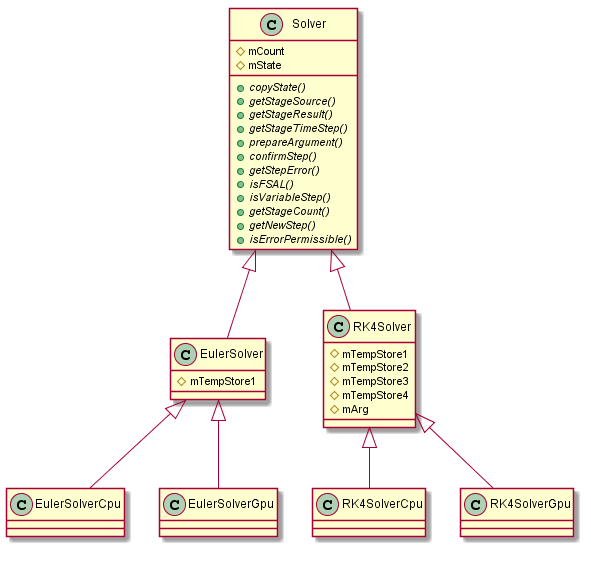
\includegraphics[width=1.0\linewidth]{solvers.png}}
	\caption{Иерархия наследования для методов численного решения}
	\label{ris:solvers}
\end{figure}

%\par EulerSolver, RK4Solver, DP45Solver являются потомками класса Solver и описывают основную информацию о реализуемых методах. Например, является ли данный численный метод методом с изменяемым шагом или требуется ли ему предварительная подготовка перед первой итерацией, сообщает количество итераций которые необходимы для данного метода (для метода Эйлера это значение равно единице). Кроме того они хранят набор констант необходимых конкретно для данного метода, например для метода Рунге-Кутты это числа, используемые при вычислении нового состояния.
% информация о методе 
%Все эти классы в полной мере реализуют все необходимые функции, описанные в классе предке, поэтому объект каждого из них можно создать. Именно они используются в качестве хранителей информации о выбранном методе решения задачи.

%\par Классы EulerSolverCpu, EulerSolverGpu и другие уже являются потомками второго уровня, они наследуются от EulerSolver, RK4Solver, DP45Solver соответственно и предназначены для работы на центральном процессоре и видеокарте соответственно. Именно эти классы в полной мере реализуют выбранный численный метод.

\par Рассмотрим подробнее работу данных классов на примере RK4SolverCpu. Экземпляр данного класса фактически является "<хранилищем"> данных. Текущее состояние хранится в mState, данное поле имеют все без исключения классы, реализующие различные численные методы. Кроме того существует несколько дополнительных "<хранилищ"> (mTempStore1, mTempStore2, mTempStore3, mTempStore4), они используются для сохранения результатов вычисления на разных стадиях. Последний подобный "<склад">  это mArg, он необходим при получении нового состояния с использованием результатов, полученных ранее при выполнении четырех стадий метода.
\par В процессе вычислений объект данного класса выдает источник данных и их приемник, для этого используются описанные ранее переменные. Например, на первой стадии в качестве источника информации будет предоставлено mState, а запишется информация в mTempStore1. Стоит отметить, что сам объект не занимается непосредственно вычислениями, это работа другого класса. После каждой стадии метода выполняется функция prepareArgument() она занимается необходимой обработкой полученных данных перед следующей итерацией метода.
\par После того, как шаг метода выполнен выполняется его подтверждение (confirmStep()), метод Рунге-Кутты является методом с постоянным шагом и никогда не отвергает полученные результаты, поэтому данная функция просто меняет местами содержимое mState и mArg, так как в последнем будет храниться новое состояние.

%Фактически подобные классы являются большими хранилищами для вычисляемых данных. Реализованный метод Рунге-Кутты предполагает четыре стадии выполнения, результат каждой стадии необходимо сохранять, а новое состояние вычисляется с использованием всех четырех результатов, полученных ранее. Данный класс при создании выделяет память под шесть матриц, которые будут использоваться при вычислениях, четыре временных хранилища, одна матрица, для текущего состояние и матрица, используемая при вычислении нового состояния. В процессе работы объект данного класса выдает в качестве источника или приемника информации либо временную матрица, либо матрицу состояния, в зависимости от текущей стадии выполнения. После завершения итерации вычисления выполняется пересчет нового состояния.

\subsection{Класс Block и его потомки}

\par Обсуждая вопрос архитектуры системы невозможно обойти одну из самых важных составляющих приложения - блоки. Область, над которой производятся вычисления, разбивается на составные части, которые и называются блоками. Для их представления используются класс Block и его потомки.

\par Класс Block является абстрактным классом и необходим для описания свойств, которые присущи всем блокам независимо от того, на каком типе устройства они будут выполняться. Например, к таким свойствам можно отнести размерность. каждый блок может быть одномерным, двумерным или трехмерным в зависимости от поставленной задачи. Кроме того каждый блок обладает определенными координатами в пространстве и размерами. Важной информацией о блоке также является тип устройства, на котором будет производится вычисление конкретно данного блока, и номер устройства, хранение этих данных тоже предусмотрена в данном классе.

\par Каждый блок должен обладать определенным набором методов, которые описаны в классе Block. К таким методам относится, например, вычисление нового состояния (computeStageCenter() и computeStageBorder()), подготовка к новой стадии численного метода (prepareArgument()), подтверждение выполненного шага и несколько других. Все эти методы позволяют полноценно работать с блоком и осуществлять вычисления.

\par Всего у класса Block существует три наследника (см. Рис.~\ref{ris:blocks}):
\begin{enumerate}
\item BlockCpu;
\item BlockGpu;
\item BlockNull.
\end{enumerate}

\begin{figure}[h]
	\center{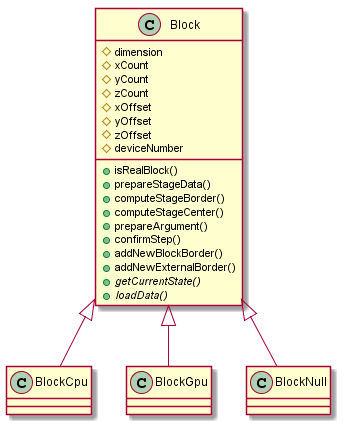
\includegraphics[width=0.7\linewidth]{blocks.png}}
	\caption{Иерархия наследования для блоков}
	\label{ris:blocks}
\end{figure}

\par Первые два класса-наследника работают на центральном процессоре и видеокарте соответственно. Как и в случае с Solver'ами подобное разделение обусловлено различными способами работы с памятью, но в данном случае это не единственная причина. В зависимости от типа устройства меняется и способ осуществления параллельных вычислений: для центрального процессора используется библиотека OpenMP, а для видеокарты язык CUDA. Подробнее это будет рассмотрено в одной из следующих глав. Объекты этих классов создают себе "<хранилища"> (наследников класса Solver) для работы с данными и реально занимаются вычислениями.

%\par Класс BlockCpu является наследником класса Block, предназначенным для работы на центральном процессоре. Он является реальным блоком, который хранит информацию и осуществляет ее обработку. Для осуществления распараллеливания используется библиотека OpenMP.

%\par Класс BlockGpu является наследником класса Block, предназначенным для работы на видеокарте. Он также является реальным блоком, но в отличии от класса BlockCpu всю информацию он хранит в памяти видеокарты, расчеты выполняются также на ней, для этого используется специальный язык CUDA.

\par BlockNull класс-наследник Block, который никаким образом не хранит данные текущем состоянии той части области, за которую он по идее отвечает. На самом деле он нужен для того чтобы обозначить, что составляющая области, относящаяся к данному блоку на самом деле обрабатывается другим потоком и на другой машине. Но он позволяет выполнить все функции присущие блоку: получение координат и размеров, даже выполнение расчетов, правда в данном случае ничего рассчитано не будет.

\par Отдельно стоит осветить вопрос пользовательских функций. Задача реализации высокого уровня  абстракции предполагала генерацию программного кода по пользовательским функциям. Наряду с областью, над которой выполняются вычисления, пользователь задает систему уравнений, которую необходимо моделировать, Кроме того задаются граничные условия. Исходя из полученных данных формируется набор пользовательских функций, которые необходимы для работы приложения. В этот набор входят функции, которые задают начальное состояние области, а также функции, позволяющие рассчитать новое значение в определенной ячейке блока.

\par Каждый блок имеет специальную матрицу, которая совпадает по размеру с количеством ячеек, относящихся к блоку. В этой матрице лежать индексы функций, которые ответственны за перерасчет конкретно данной ячейки. На этапе подготовки выполняет компиляция пользовательских функций и формирования списка указателей на них. Индексы из этого списка и заносятся в матрицу. Функция для любой ячейки имеет унифицированную сигнатуру, что позволяет удобным образом осуществлять ее вызов, не задумываясь об особом статусе ячейки, если таковой имеет место быть.

%Основными классами приложения, которые занимаются непосредственно вычислениями на устройствах, являются потомки класса Block - BlockCpu и BlockGpu. Как можно догадаться из названия данных классов они предназначены для выполнения вычислений на центральном процессоре и видеокарте соответственно. Кроме того присутствует класс BlockNull, который не выполняет вычислительной функции, а лишь хранит общую информацию о блоке, необходимую для корректной работы.

%\par Классами, которые определяют численные методы решения задачи, являются потомки класса Solver, например EulerSolver, RK4Solver или DP45Solver, эти классы хранят минимальный набор информации о методе Эйлера, методе Рунге-Кутты четвертого порядка и семистадийном методе Дормана-Принса. Их потомки, например EulerSolverCpu и EulerSolverGpu, создаются на центральном процессоре и видеокарте соотвественно и являются полноценной реализацей методов для работы на представленных устройствах.

\subsection{Класс Interconnect}

%\par Для пересылки данных между блоками, который расположены на разных узлах вычислительного кластера используется класс Interconnect. Каждый его экземпляр хранит номер потока, являющегося источником передаваемой информации, номер потока, который данную информацию должен принять, а также длину массива, который необходимо переслать. Экземпляры этого класса создаются на каждую связь между блоками каждым потоком. При вызове функции передачи/приема объект выполнит либо отправку сообщения, либо прием в зависимости от номера потока, который вызвал данную функцию у себя, либо не будет выполнено ничего, если пересылка осуществляться не должна, например поток не имеет к ней вообще никакого отношения, не является ни источником, ни приемником, либо пересылка для данной связи не требуется - блоки принадлежат одному потоку и, как следствие, расположены на одной машине и могут получать данные напрямую.

\par В процессе вычислений блокам требуется информация, которую необходимо получить от других составляющих области. Поэтому в контексте рассмотрения класса для передачи информации между блоками полезно заострить внимание на особенностях, связанных с их размещением. Очевидно, что существует три варианта размещения каждой пары блоков друг относительно друга:
\begin{enumerate}
\item блоки располагаются на одном вычислительном устройстве;
\item блоки размещаются на разных устройствах в пределах одной машины;
\item блоки находятся на разных машинах.
\end{enumerate}

\begin{figure}[h]
	\begin{minipage}[h]{0.3\linewidth}
		\center{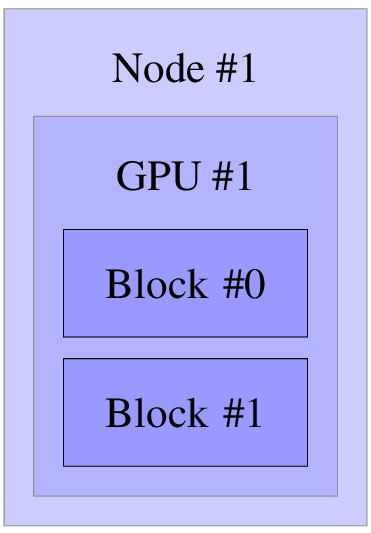
\includegraphics[width=0.7\linewidth]{1Node_1Device_2Block.png} \\ Одно устройство}
	\end{minipage}
	\hfill
	\begin{minipage}[h]{0.6\linewidth}
		\center{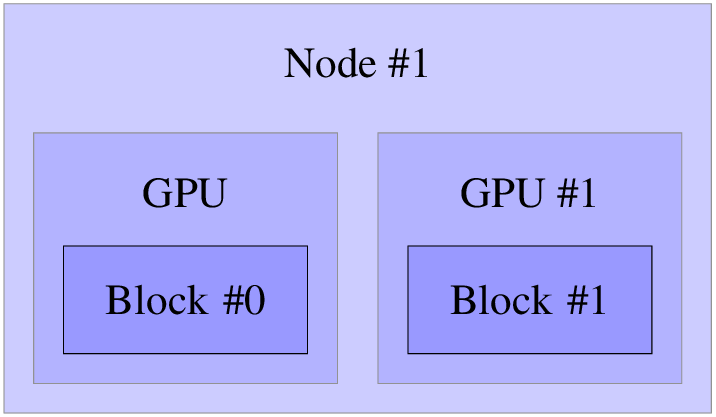
\includegraphics[width=0.85\linewidth]{1Node_2Device_2Block.png} \\ Два устройства на одной машине}
	\end{minipage}
	\hfill
	\begin{minipage}[h]{1.0\linewidth}
		\center{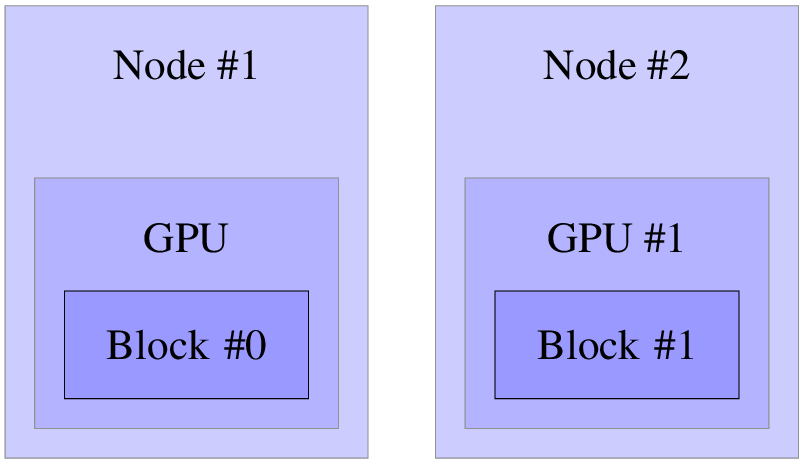
\includegraphics[width=0.6\linewidth]{2Node_2Device_2Block.png} \\ Два устройства на разных машинах \\ ~ }
	\end{minipage}
	\caption{Варианты расположения блоков}
	\label{ris:var}
\end{figure}

\par В случае расположения блоков на одном вычислительном устройстве проблема обеспечения доступа одного блока к данным, складируемой другим, фактически отсутствует, так как в данной ситуации нет ограничения для доступа к памяти.

\par Во втором случае существуют ограничения вызванные тем, что центральный процессор не имеет возможности напрямую читать из памяти видеокарты, ровно как и видеокарта не может осуществлять подобные манипуляции с памятью центрального процессора. Данная проблема решается путем выделения памяти под данные, которые необходимы другим блокам, в специальной области, доступ к которой имеют оба вида вычислительных устройств.

\par Основные трудности связаны с передачей информации в третьем случае. Расположения блоков на разных машинах гарантирует невозможность прямого обращения к памяти и получения информации. Для решения данной проблемы и создан класс Interconnect. Объекты данного класса используются для пересылки данных между блоками, который располагаются на различных узлах вычислительного кластера. Каждый экземпляр хранит номер потока, являющегося источником информации, то есть потока, в которому реально приписан интересующий нас блок. Кроме того хранится номер потока приемника информации, такой потом тоже содержит реальный блок, которому необходима данная информация. Также каждый объект класса Interconnect знает длину массива передаваемой информации, это необходимо для корректной работы библиотеки MPI, которая используется для передачи данных.

\par Экземпляры данного класса создаются на каждую связь между блоками всеми потоками исполнения независимо от того относятся ли зависимые блоки к данным потокам. При вызове функции передачи/приема экземпляр класса выполнит либо отправку сообщения с данными, либо их прием в зависимости от номера потока, который вызвал данную функцию у себя, либо не будет выполнено ничего, если пересылка осуществляться не должна, например поток не имеет к ней вообще никакого отношения, не является ни источником, ни приемником, либо пересылка для данной связи не требуется - она относится к первым двум случаям.

%\par Стоит отметить, что среди всех потоков выполнения главным считает поток с номером 0. Именно он собирает со всех данные и выполняет их сохранение, он же отвечает за вывод конечного результата вычислений, Кроме того он также участвует в вычислениях наряду с другими потоками.

\subsection{Класс Domain}

\par Главным управляющим классом приложения является класс Domain. Объект данного класса создается в единственном экземпляре каждым потоком. Предполагается, что на одном вычислительном узле не запускается более одного потока. Подобное ограничение введено с целью исключить следующую ситуацию. На одной машине одновременно выполняются два или более потоков. Каждый из них имеет некоторое количество блоков и вполне вероятно, что некоторые блоки, принадлежащие разным потокам, окажутся на одном вычислительном устройстве. Кроме того очевидно, что все блоки располагаются в пределах одной машины. Как было описано ранее в подобной ситуации передача данных между блоками средствами библиотеки MPI не требуется, так как ее можно организовать проще и. что еще более важно, она может осуществляться быстрее. Но в случае, который сейчас рассматривается, передача информации будет осуществлять именно через стороннюю библиотеку. С целью предотвращения подобной ситуации и было введено данное ограничение, которое фактически не мешает полноценному функционированию приложения.

\par Объекты класса Domain, как было сказано ранее, осуществляют управление вычислениями, каждый на своем потоке. В начале выполнения считывается файл, содержащий всю необходимую информацию о решаемой задаче: количество блоков, их размерность, размеры и координаты, а также данные о связях между блоками и другие сведения. Все это позволяет полностью сформировать набор переменных для дальнейшего решения (см. Рис.~\ref{ris:all}). Основную часть этих переменных, конечно, составляют блоки и связи между ними. Кроме того здесь же выполняется присвоение значений таким переменным как номер потока выполнения, количество потоков в целом, количество блоков и соединений. Также создается объект класса-наследника Solver, который будет предоставлять необходимую информацию о численном методе, применяющемся для решения задачи.
\begin{figure}[h]
	\center{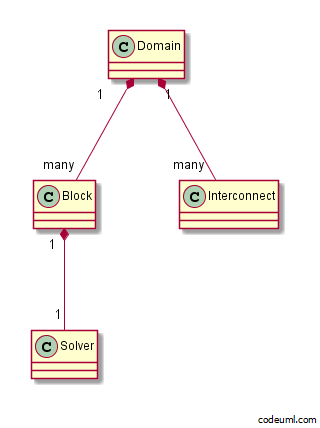
\includegraphics[width=0.55\linewidth]{all.png}}
	\caption{Общая архитектура приложения}
	\label{ris:all}
\end{figure}

\subsection{Схема работы приложения}

\par Прежде чем переходить к рассмотрению схемы работы приложения (см. Рис.~\ref{ris:scheme}) необходимо ввести понятия центральных и граничных элементов блока.

\begin{figure}[h]
	\center{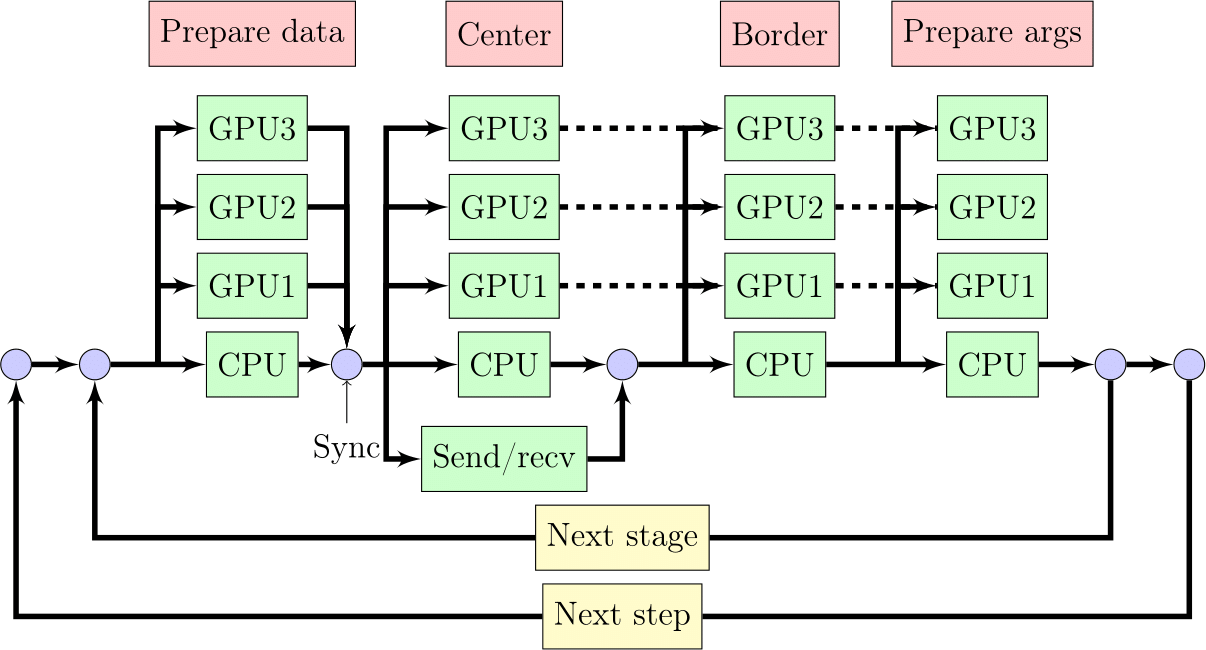
\includegraphics[width=1.0\linewidth]{scheme.png}}
	\caption{Схема вычислений}
	\label{ris:scheme}
\end{figure}

\par Центральными элементами будем называть такие элементы, для вычисления новых значений которых не требуется данных от других блоков.

\par Граничные элементы - это элементы, для вычисления новых значений которых могут потребоваться данные от других блоков, следовательно не исключена возможность пересылки данных между различными вычислительными узлами кластера.

\par После того, как выполнена полная инициализация задачи можно начинать вычисления. На каждом потоке объект управляющего класса вызывает функцию compute(), которая начинает вычисления. До тех пор, пока не будет выполнено необходимое условие будут выполнять действия представленные на Рис.~\ref{ris:scheme}. Сначала каждый блок выполняет подготовку данных, то есть копирует часть своей информации, которая нужна его  "<соседям"> - блокам, с которыми у него есть связь. Подобные действия выполняет каждый блок на каждой машине.

\par Важной опорной элементом алгоритма является точка синхронизации. В этом момент времени можно быт уверенным, что все потоки пришли в эту точку и дождались друг друга. Это необходимо для того чтобы потоки не обгоняли друг друга. Например, область состоит из двух блоков, но один из них оказался значительно больше другого. В такой ситуации поток. работающий с блоком меньшего размера, будет выполнять вычисления значительно быстрее, будет предоставлять некорректные данные для пересылки и решение в конечном итоге окажется неверным. Для исключения подобной ситуации введена синхронизация потоков. Важно отметить, что инициализация новых вычислений или подготовки данных на центральном процессоре невозможно до завершения предыдущих действий, а каждый возов вычислений на ядре видеокарты всегда дожидается завершения предыдущего вызова на этой видеокарте.

\par После завершения этих действий мы имеем полностью подготовленные массивы, которые и будут пересылаться между вычислительным узлами кластера. Если пересылка не требуется, блоки расположены в пределах одной машины, то брать информацию будут именно из этих массивов напрямую, иначе инициализируется процесс пересылки данных. Данное действие требует значительных временных затрат, которые вполне разумно использовать для вычисления той части блоков, которым пересылаемые данные не могут потребоваться в Принсипе - центральных блоков. В связи с этим передача данных выполняется асинхронным образом, то есть после вызова команды "<отправить"> процесс, вызвавший ее, не дожидается завершения операции, а продолжает работу. Аналогичным образом поступает и поток, который информацию будет принимать, он просто сигнализирует о том, что готов это сделать, но не дожидается окончания передачи данных. Пока информация пересылается и ведется расчет центральных элементов. Вычисления запускаются одновременно на центральном процессоре и видеокартах. Каждое устройство будет выполнять вычисления только с блоками, которые принадлежать этому устройству. Если окажется, что таких блоков нет, то устройство просто завершит выполнения данной части алгоритма.

\par После того, как процессор завершил расчет центральных элементов, относящихся к его блокам, он запускает ожидание окончания пересылки. Так как передача данных выполнялась асинхронным образом обязательно нужно убедиться, что действие завершено, прежде чем приступать к вычислению граничных элементов, новые значения которых могут зависеть от этих данных. Данные вычисления осуществляются аналогично вычислениям центральных элементов.

\par Далее необходимо выполнить подготовку аргументов, ведь если мы используем многостадийный метод нам вполне может потребоваться, например, сумма матриц, полученных на предыдущих стадиях, а это дополнительные вычисления, которые можно и нужно распараллелить. Затем мы либо отправляемся выполнять следующую стадию метода, либо переходим к следующей итерации - выполняем шаг по времени. И все это длится до тех пор, пока либо мы не достигнем заданных условий, либо пользователь не остановит процесс принудительно.

\section{Компоненты программного комплекса}

\subsection{Общие сведения}

\par Важной составляющей программного комплекса, ориентированного на конечного пользователя является пользовательский интерфейс. В его задачи входит предоставление удобных инструментов для управления задачами и вычислениями, а именно: создание и сохранение проектов, запуск, приостановка и завершение вычислений, визуализация полученных результатов.

\par Значимую роль в работе приложения играет программа предварительной обработки. Данная часть комплекса ответственна за преобразование пользовательских функций в код, который впоследствии будет скомпилирован и использован при расчетах. Кроме того данная часть приложения разбивает область задачи на блоки и осуществляет их распределение по вычислительным устройствам и узлам кластера, а также создает бинарный файл со всей необходимой информацией, который передается вычислительному ядру для дальнейшей работы и вычислений на его основе.

\par Наконец, параллельный фреймворк или вычислительное ядро занимается непосредственно распределенными вычислениями. В задачи этой части программного комплекса входит непосредственно осуществление параллельного выполнения расчетов на вычислительном кластере.

%\par Приложение состоит из нескольких частей. Каждая из них отвечает за определенную часть работы, либо подготовительной, либо относящейся непосредственно к самим вычислениям, либо реализующей взаимодействие с пользователем.

%\par Пользовательский интерфейс позволяет создавать и модифицировать проекты. Кроме того он дает возможность управлять текущими вычислениями, а именно запускать, прекращать, приостанавливать, а также выполнять сохранение текущего состояния и его загрузку.

%\par Часть предварительной обработки выполняет подготовку исходных данных. В ней происходит обработка геометрии и свойств области, производится определение размерности, расположения и размера блоков, граничных условий. Здесь же выполняется распределение блоков по вычислительным устройствам, формируется библиотека пользовательских функций.

%\par Параллельный фреймворк и алгоритмы обработки данных составляют основу приложения и занимаются непосредственно самими вычислениями. К алгоритмам обработки данных относятся метод Эйлера, явные схемы Рунге-Кутты, методы Дормана-Принса. Стоит отметить, что присутствует возможность расширения списка доступных методов решения.

\subsection{Параллельный фреймворк}

%\par Параллельный фреймворк занимается непосредственной реализацией распределенных вычислений. С его помощью выполняется взаимодействие всех вычислительных устройств во время работы приложения. Он же реализует пересылку данных между блоками. Подобные пересылки необходимы в случае, когда одному блоку нужна информация от другого для продолжения собственных вычислений. Кроме того фреймворк занимается обработкой событий, которые генерирует пользовательский интерфейс, а именно начало вычислений с заданными параметрами, приостановка вычислений, их прекращении, сохранение и загрузка состояний.

\par Поговорим чуть подробнее о механизмах и инструментах, которые используются при распределенных вычислениях. Фактически распараллеливание проводится в два этапа:
\begin{enumerate}
\item разделение задачи на блоки - крупнозернистый параллелизм;
\item параллельные вычисление на устройстве - мелкозернистый параллелизм.
\end{enumerate}

\subsubsection{Крупнозернистый параллелизм}

\par Крупнозернистый параллелизм осуществляется путем разбиения области на блоки и распределения блоков по вычислительным устройствам еще на этапе подготовки, о чем было изложено ранее. Данный подход позволяет использовать все вычислительные мощности имеющиеся в наличии и равномерно распределять нагрузку на устройства. На одном устройстве может располагаться несколько блоков одновременно, в таком случае их вычисление будет осуществляться в порядке очереди. Немаловажным фактом является то, что в случае если количество блоков значительно (в несколько раз) превышает количество вычислительных устройств, то блоки, которые имеют общие границы разумно располагать на одном устройстве, либо в пределах одной машины, а блоки не имеющих таких границ - на разных, сохраняя равномерность распределения блоков по устройствам в целом. Такой подход позволяет увеличить скорость расчетов для небольших, по количеству используемых узлов, областей. Достигается это уменьшение времени, которое необходимо на пересылку данных между блоками между итерациями вычислений, так как если блоки расположены на одном вычислительном устройстве или одной машине, то пересылка не будет выполняться в Принсипе, потому что данные уже доступны блоку. Очевидно, что в общем случае невозможно распределить все блоки таким образом чтобы пересылок не было вообще, но такой подход позволяет минимизировать количество пересылаемой информации, что положительно сказывается на производительности.

\subsubsection{Мелкозернистый параллелизм}

\par Мелкозернистый параллелизм осуществляется непосредственно на вычислительных устройствах. В зависимости от типа устройства будет использована библиотека OpenMP, для работы на центральном процессоре, и CUDA, в случае работы на видеокарте. Увеличение производительности достигается путем параллельного вычисления частей блока.

\par OpenMP реализует параллельные вычисления с помощью многопоточности, в которой "<главный"> (master) поток создает набор подчиненных (slave) потоков и задача распределяется между ними. Предполагается, что потоки выполняются параллельно на машине с несколькими процессорами (количество процессоров не обязательно должно быть больше или равно количеству потоков). Количество создаваемых потоков может регулироваться как самой программой при помощи вызова библиотечных процедур, так и извне, при помощи переменных окружения.

\par Данная библиотека работает в системах с общей памятью, поэтому каждая нить имеет доступ ко всем данным блока. Например, при расчете двумерного случая прямоугольник "<разрезается"> на полосы, обработка которых осуществляется одновременно. Библиотека OpenMP самостоятельно определяет количество таких полос и их ширину.

\par В качестве аналога данной библиотеки можно было использовать стандартные потоки языка C++, но подобный подход значительно усложнил бы разработку и увеличил вероятность ошибки. OpenMP обладает всеми необходимыми инструментами для реализации многопоточности на центральном процессоре в рамках одной машине и достаточно проста в использовании.

%\par Конкретно в данным случае библиотека осуществляет распараллеливание расчетов нового состояния блока. Каждой нити исполнения дается на обработку часть матрицы. Нить выполняет расчет новых значений основываясь на текущих данных своей части, кроме того она имеет возможность получить данные, которые обрабатывают другие нити, если таковые потребуются для расчета своих значений. Так как работа ведется с общей памятью никакой подготовки для такого "<чтения"> не требуется.

\par Как уже сообщалось ранее, при осуществлении вычислений на видеокарте используется CUDA - (Compute Unified Device Architecture) программно-аппаратная архитектура параллельных вычислений, которая позволяет существенно увеличить вычислительную производительность благодаря использованию графических процессоров фирмы Nvidia.

\par CUDA SDK позволяет программистам реализовывать на специальном упрощённом диалекте языка программирования Си алгоритмы, выполнимые на графических процессорах Nvidia, и включать специальные функции в текст программы на Си. Архитектура CUDA даёт разработчику возможность по своему усмотрению организовывать доступ к набору инструкций графического ускорителя и управлять его памятью.

\par При обработке блока на видеокарте каждая ячейка блока обрабатывается отдельным потоком. Каждый такой поток имеет необходимый доступ к данным.

\par В качестве альтернативы CUDA можно рассмотреть OpenCL, данный фреймворк для работы с графическими процессорами также предоставляет необходимые инструменты. Но так как CUDA разработана компанией Nvidia специально для своих видеокарт и, как следствие, она демонстрирует лучшие показатели производительности именно на видеокартах данной торговой марки. На вычислительный кластеры ставят подобные видеокарты, поэтому в качестве инструмента работы с видеокартами была выбрана именно CUDA.

\subsubsection{Передача информации между узлами}

\par Пересылка данных между разными машинами (вычислительными узлами) осуществляется с помощью библиотеки MPI. Message Passing Interface (MPI, интерфейс передачи сообщений) - программный интерфейс (API) для передачи информации, который позволяет обмениваться сообщениями между процессами, выполняющими одну задачу. MPI является наиболее распространённым стандартом интерфейса обмена данными в параллельном программировании, существуют его реализации для большого числа компьютерных платформ. Используется при разработке программ для кластеров и суперкомпьютеров. Основным средством коммуникации между процессами в MPI является передача сообщений друг другу. В стандарте MPI описан интерфейс передачи сообщений, который должен поддерживаться как на платформе, так и в приложениях пользователя. В первую очередь MPI ориентирован на системы с распределенной памятью, то есть когда затраты на передачу данных велики.

\section{Тестирование}
33333
\section{Список литературы}

\begin{thebibliography}{99}

\bibitem{pr_first}
\textit{Круглов В.\,В., Борисов В.\,В. } 
{Искусственные нейронные сети. Теория и практика. 
М.: Горячая линия - Телеком, 2001. — 382 с. } 

\bibitem{pr_second}
\textit{Кохонен Т. } 
{Ассоциативные запоминающие устройства. 
М.: Мир, 1982. — 384 с. } 

\bibitem{pr_third}
\textit{Колесов А.\;Ю., Колесов Ю.\;С. } 
{Релаксационные колебания в математических моделях экологии. 
М., 1993 (Тр. МИАН. Т. 199).}

\bibitem{pr_forth}
\textit{Глызин С.\,Д., Колесов А.\,Ю., Розов Н.\,Х. } 
{Релаксационные автоколебания в нейронных системах. I
// Дифференциальные уравнения. 2011. Т. 47, № 7. С. 919 – 932. } 

\bibitem{pr_fifth}
\textit{Глызин С.\,Д., Колесов А.\,Ю., Розов Н.\,Х. } 
{Релаксационные автоколебания в нейронных системах. II
// Дифференциальные уравнения. 2011. Т. 47, № 12. С. 1675 – 1692. } 

\bibitem{pr_sixth}
\textit{Глызин С.\,Д., Колесов А.\,Ю., Розов Н.\,Х. } 
{Релаксационные автоколебания в нейронных системах. III
// Дифференциальные уравнения. 2012. Т. 48, № 2. С. 155 – 170. }

\bibitem{pr_seventh}
\textit{Кащенко С.\,А., Майоров В.\,В.\, } 
{Модели волновой памяти. 
М.: Либроком, 2009. — 288 с. }  

\bibitem{pr_eighth}
\textit{Глызин С.\,Д., Колесов А.\,Ю., Розов Н.\,Х. } 
{Дискретные автоволны в нейронных системах.
Журнал вычислительной математики и математической физики. 2012. Т. 52, № 5. С. 840–858. } 

\bibitem{pr_nineth}
\textit{Глызин С.\,Д., Колесов А.\,Ю., Розов Н.\,Х. } 
{Моделирование эффекта взрыва в нейронных системах.
// Математические заметки. 2013. Т. 93, № 5. С. 682–699. } 

\bibitem{pr_tenth}
\textit{Боресков А.\;В., Харламов А.\;А. } 
{Основы работы с технологией CUDA. 
М.: ДМК Пресс, 2010. — 232 с. } 

\bibitem{pr_eleventh}
\textit{Антонов А.\,С. } 
{Параллельное программирование с использованием OpenMP. 
М.: Изд-во МГУ, 2009. - 77 с. } 

\bibitem{pr_twelveth}
\textit{Сандерс Дж., Кэндрот Э. } 
{Технология CUDA в примерах. Введение в программирование графических процессоров. 
М.: ДМК Пресс, 2013. — 232 с. } 

\bibitem{pr_fourteenth}
\textit{Горелов Ю.\,Н. } 
{Численные методы решения решения обыкновенных дифференциальных уравнений (метод Рунге-Кутта).
Самара: Самарский университет, 2006. — 48 с. } 

\bibitem{pr_fifteenth}
\textit{Ивановский Л.\;И., Самсонов С.\;О. } 
{Фазовые перестройки одной двумерной динамической системы с импульсным воздействием.
// Модел. и анализ информ. систем, 2014. Т. 21, №6. С. 179 – 181. } 

\bibitem{pr_sixteenth}
\textit{Гукенхеймер Дж., Холмс Ф. } 
{Нелинейные колебания, динамические системы и бифуркации векторных полей. 
Москва-Ижевск.: Институт компьютерных исследований, 2002. – 560 с. } 

\bibitem{pr_seventeenth}
\textit{Арнольд В.\;И. } 
{Дополнительные главы теории обыкновенных дифференциальных уравнений. 
М.: Наука, 1978. — 304 с. } 

\end{thebibliography}


%Для автоматизации моделирования конечно-разностных диффузионных систем необходимо решить несколько задач. Среди них разработка инструмента моделирования уравнений (в том числе и уравнений с запаздыванием), которые были бы распределены в одномерных, двумерхных и трехмерных областях. Каждая область может быть представлена неким набором блоков. Для одномерного случая этими блоками являются отрезки, в случае плоскости - прямоугольник и, если область является трехмерной - параллелепипеды. Каждый из блоков характеризуется своими координатами в пространстве, размерами и информацией о своих границах. Граница блока может быть составлена из нескольких частей  Дирихле Нейман граница с другим блоком. РИСУНКИ Кроме того нужна поддержка соверенного оборудования , а именно неоднородных систем с иерархической организацией памяти. Также требуется высокий уровень абстракции, такой как автоматическая генерация кода по пользовательским функциям.  пользовательский интерфейс.
\end{document}


















